\subsubsection{Módulo GPS}


El sistema utiliza el módulo GPS GY-NEO6MV2 para determinar la posición y velocidad del material rodante. Este módulo basado en el chip NEO-6M se alimenta con 5V y permite la comunicación con el MCU a través de una interfaz UART. Sin embargo, no cuenta con una entrada de reset y a partir de experiencias previas de otros proyectos con módulos de estas características, se decidió armar un circuito de reset externo por en caso de detectar un error o falla en el funcionamiento del módulo. \\ 

El circuito de reset utilizado se puede observar en la figura \ref{fig:gps_sch} y utiliza el transistor MOSFET de canal P SI2343DS-T1-E3 de Vishay Semiconductors \cite{SI2343DS-T1-E3} diseñado para aplicaciones de conmutación y  control de carga en circuitos de baja potencia. Tiene una baja resistencia de encendido Rds(on) lo que permite generar una pequeña caída de tensión respecto a los 5V que se buscan llevar al módulo. Para polarizar el circuito y permitir la circulación de corriente para encender el módulo, se debe forzar la entrada GPS\_PW\_ON a su estado bajo de 0V. Para cortar la circulación de corriente y apagar el módulo, se debe colocar la entrada en estado de alta impedancia; esto se logra configurándolo como un pin de entrada.\\ 

\begin{figure}[H]
    \centering
    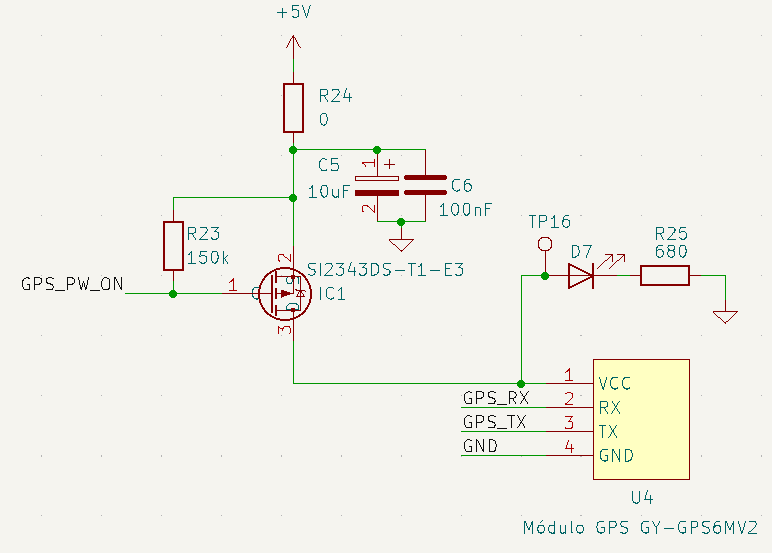
\includegraphics[width = 0.8 \linewidth]{img/gps_sch.png}
    \caption{Circuito de reset del módulo GPS}
    \label{fig:gps_sch}
\end{figure}    

Además, se agregó un LED con su respectiva resistencia para indicar cuando el módulo está alimentado y cuando no lo está, ya que el módulo no trae integrado ningún indicar luminoso. También se colocaron dos capacitores de desacople, uno electrolítico de 10 $\mu$F y otro cerámico de 100nF para filtrar los ruidos que pueda haber en la línea de alimentación considerando también que es un módulo que trabaja con altas frecuencias y genera mayor ruido. 
